\section[Problématique]{Problématique}

\subsection[Apprentissage statistique]{Apprentissage statistique}

\begin{frame}{Réduction de dimensions en régression linéaire}
	Nous avons vu dans le chapitre sur la régression linéaire que le problème d'apprentissage statistique devient \textbf{mal formé} lorsque les caractéristiques d'entrée du problème $x \in \mathcal{X}$ sont \textbf{linéairement dépendantes}:
	\begin{itemize}
		\item La matrice $\tilde{X}$ n'est pas de plein rang de colonnes.
		\item La matrice $\tilde{X}^T \tilde{X}$ n'est pas de plein rang et n'est donc pas inversible.
		\item Il existe plusieurs solutions au problème $\tilde{X}^T \tilde{X} \beta = \tilde{X}^T Y$
	\end{itemize}
\end{frame}

\begin{frame}{Réduction de dimensions en apprentissage statistique}
	\begin{itemize}
		\item La \textbf{stricte} dépendance linéaire est donc un problème fondamental pour la résolution du problème de régression linéaire.
		\pause 
		\item Plus largement, utiliser en entrée d'un algorithme d'apprentissage statistique des caractéristiques d'entrée \textbf{fortement corrélées} entre elles est discutable. En effet, quel intérêt pour notre algorithme d'apprendre à partir d'informations \textit{redondantes} ? Cela complexifie le modèle (et donc augmente la variance) pour un bénéfice limité.
		\pause
		\item L'\textbf{Analyse en Composante Principale} apporte justement une solution à ce problème en analysant les \textbf{inter-dépendances} entre les caractéristiques d'entrée du problème.
	\end{itemize}
\end{frame}

\begin{frame}{Une solution évidente. Vraiment ?}
	\begin{itemize}
		\item Nous avons précédemment vu que si 2 (ou plus) caractéristiques d'entrée sont linéairement dépendantes ou fortement corrélées, alors il suffit de choisir \textit{l'une d'elles} comme entrée à notre problème.
		\pause
		\item C'est correct, mais peu satisfaisant: \textit{laquelle} précisément ?
		\pause
		\item L'analyse en composante principale propose de prendre une \textbf{combinaison linéaire} de ces mêmes caractéristiques.
	\end{itemize}
\end{frame}

\subsection[Idée générale de l'ACP]{Idée générale de l'ACP}

\begin{frame}{Combinaison linéaire de caractéristiques d'entrée}
	Si le problème d'apprentissage dispose d'un espace des caractéristiques d'entrée $\mathcal{X} \subset \R^p$, une combinaison linéaire des  caractéristiques d'entrée $x^{(i)} \in \mathcal{M}_{1,p}(\R)$ pour une observation $i$ est donnée par:
	\begin{equation}
		z^{(i)} = u_1 x_1^{(i)} + u_2 x_2^{(i)} + \cdots + u_p x_p^{(i)} = x^{(i)} u
		\nonumber
	\end{equation}
	\pause
	Avec $z$ un \textbf{score} qui combine plusieurs caractéristiques et $u \in \mathcal{M}_{p,1}(\R)$. Un score $Z \in \mathcal{M}_{n,1}(\R)$ peut alors être calculé pour l'ensemble des données $X \in \mathcal{M}_{n,p}(\R)$:
	\begin{equation}
		Z = X u
		\nonumber
	\end{equation}
\end{frame}

\begin{frame}{Projection des observations}
	Cela revient à \textbf{projeter} les observations sur une droite $D$ de vecteur directeur $u$. Les coordonnées des points \textbf{projetés} $\hat{X}$ dans la base $\mathcal{B}$ de $\mathcal{X}$ s'écrivent:
	\begin{equation}
		\hat{X} = Z u^T = X u u^T
		\nonumber
	\end{equation}
	\pause
	\begin{columns}
		\begin{column}{0.4\textwidth}
			\begin{itemize}
				\item $Z$ est un scalaire représentant la distance entre l'origine et la projection le long de la droite $D$.
				\item L'\textbf{erreur} est définie comme le vecteur entre la projection sur $D$ $\hat{X}$ et de son point d'origine $X$.
			\end{itemize}
		\end{column}
		\begin{column}{0.6\textwidth}
			\begin{figure}
				\centering
				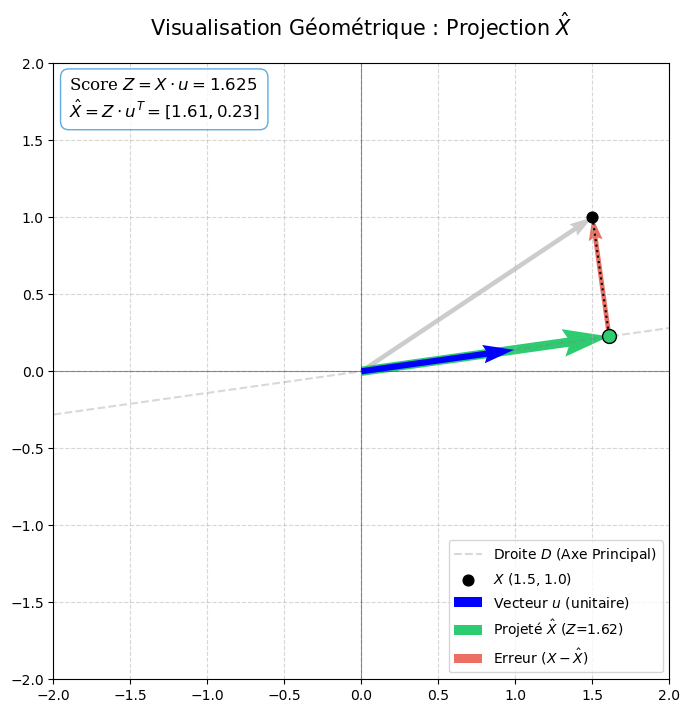
\includegraphics[height=0.75\linewidth]{Images/projection}
				\label{fig:projection}
			\end{figure}
		\end{column}		
	\end{columns}
\end{frame}

\begin{frame}{Composante principale}
	On cherche une droite $D$ et un vecteur directeur $u$ particuliers. L'objectif de l'analyse en composante principale consiste à choisir $u$ de telle sorte que la variance du score $Z$ soit \textbf{maximale}. Cela revient à choisir une droite $D$ qui minimise les erreurs $X - \hat{X}$. \\
	\vspace{0.5cm}
	\pause
	Cette droite ne \textbf{doit pas} être confondue avec la droite de régression linéaire liant les caractéristiques. Par exemple, avec $\mathcal{X} \subset \R^2$:
	\begin{figure}
		\centering
		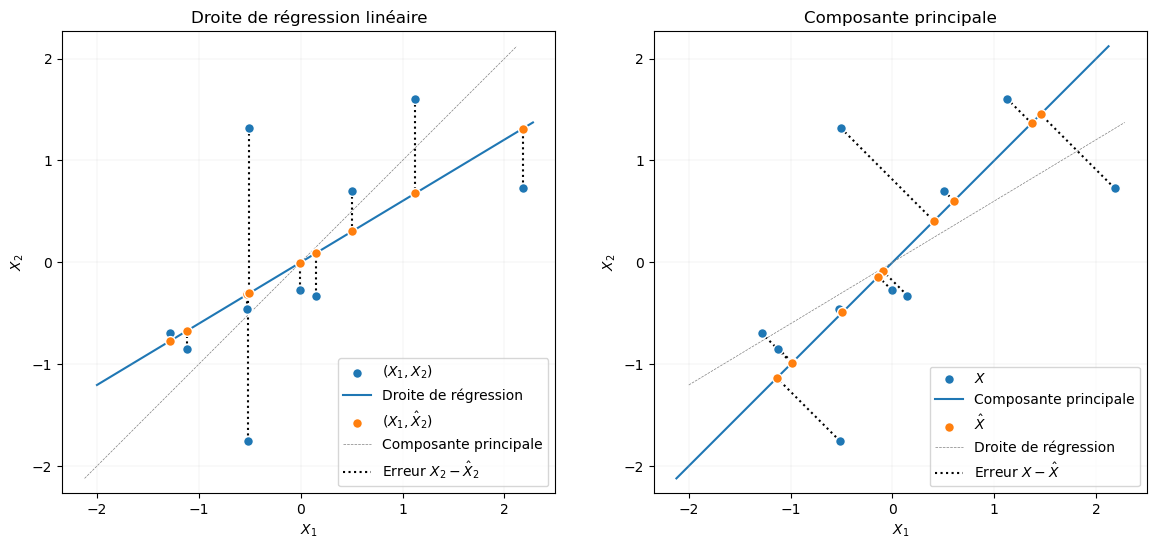
\includegraphics[width=0.85\linewidth]{Images/regression_vs_projection}
		\label{fig:regression_vs_projection}
	\end{figure}
\end{frame}

\subsection[Formulation du problème]{Formulation du problème}

\begin{frame}{Données d'apprentissage standardisées}
	Dans l'analyse en composantes principales, nous nous intéressons à des caractéristiques d'entrée $x \in \R^p$ \textbf{centrées} et de variances \textit{similaires}. Une façon de s'assurer du centrage et de la similarité de la variance consiste à \textbf{standardiser} les variables $x_j$ de telle sorte que sur les données d'apprentissage $\mathcal{D} = \{x^{(i)}\}_{i=1}^n$:
	\pause
	\begin{equation}
		\begin{aligned}
			\bar{X}_{\bigdot j} &= \displaystyle \frac{1}{n} \sum_{i=1}^n x_j^{(i)} = 0 \quad \forall j=1, 2, \dots, p \\
			\Varhat{X_{\bigdot j}} &= \displaystyle \frac{1}{n} \sum_{i=1}^n (x_j^{(i)} - \bar{X}_{\bigdot j})^2 = 1 \quad \forall j=1, 2, \dots, p
		\end{aligned}
		\nonumber
	\end{equation}
	\pause
	Avec $X_{\bigdot j}$ la $j$\textsuperscript{ème} colonne de $X$. Dans le contexte de l'ACP, on néglige la correction de Bessel, on travaille donc avec des estimateurs biaisés. Mais cela n'a pas de conséquence sur la déterminations des composantes principales.
\end{frame}

\begin{frame}{Optimisation sous contrainte pour la première composante principale}
	La première composante principale, représentée par la droite $D_1$ de vecteur unitaire $u_1 \in \mathcal{M}_{p,1}(\R)$ est obtenue pour un vecteur $u_1$ maximisant la variance du score $z_1$. Nous imposons une contrainte afin que $u_1$ soit un vecteur unitaire:
	\begin{equation}
		\argmax{u_1 \in \mathcal{M}_{p,1}(\R)} \Varhat{Z_1} \quad \text{s.c} \quad \|u_1\|_2^2 = 1
		\nonumber
	\end{equation}
	Avec:
	\begin{equation}
		Z_1 = X u_1
		\nonumber
	\end{equation}
	Nous recherchons la variance maximale de $Z$ afin d'expliquer la relation $Y \mid X$ de notre problème d'apprentissage statistique (régression ou classification).
\end{frame}

\begin{frame}{Simplification du problème d'optimisation}
	Puisque les données d'apprentissage $X$ sont centrées:
	\begin{equation}
		\begin{aligned}
			\bar{Z}_1 
			&= \frac{1}{n} \sum_{i=1}^n z_1^{(i)} \\
			&= \frac{1}{n} \sum_{i=1}^n \left(x^{(i)} u_1\right) \\
			&= \left(\frac{1}{n} \sum_{i=1}^n x^{(i)}\right) u_1 \\
			&= \frac{1}{n} \bar{X} u_1 \\
			&= 0
		\end{aligned}
		\nonumber
	\end{equation}
	Avec $\bar{X} \in \mathcal{M}_{1,p}(\R)$ qui représente la moyenne des colonnes de $X$. 
\end{frame}

\begin{frame}{Simplification du problème d'optimisation}
	\begin{equation}
		\begin{aligned}
			\Varhat{Z_1} 
			&= \frac{1}{n} \sum_{i=1}^n \left(z_1^{(i)} - \bar{Z}_1\right)^2 \\
			&= \frac{1}{n} \sum_{i=1}^n \left(z_1^{(i)}\right)^2 \\
			&= \frac{1}{n} Z_1^T Z_1 \\
			&= \frac{1}{n} (X u_1)^T (X u_1) \\
			&= \frac{1}{n} u_1^T X^T X u_1
		\end{aligned}
		\nonumber
	\end{equation}
\end{frame}

\begin{frame}{Simplification du problème d'optimisation}
	La matrice de covariance sur les colonnes de $X$ dispose des éléments suivants pour tout $i=1, 2, \dots p$ et tout $j=1, 2, \dots, p$:
	\begin{equation}
		\begin{aligned}
			\Covhat{X_{\bigdot i}, X_{\bigdot j}} 
			&= \E{\left(X_{\bigdot i} - \E{X_{\bigdot i}}\right)^T \left(X_{\bigdot j} - \E{X_{\bigdot j}}\right)} \\
			&= \E{X_{\bigdot i}^T X_{\bigdot j}} \\
			&= \frac{1}{n} X_{\bigdot i}^T X_{\bigdot j}
		\end{aligned}
		\nonumber
	\end{equation}
	\pause
	On note $\Sigma$ la matrice de covariance des colonnes de $X$:
	\begin{equation}
		\Sigma = \frac{1}{n} X^T X
		\nonumber
	\end{equation}
\end{frame}

\begin{frame}{Simplification du problème d'optimisation}
	La variance de $Z_1$ devient donc:
	\begin{equation}
		\begin{aligned}
			\Varhat{Z_1} 
			&= \frac{1}{n} u_1^T X^T X u_1 \\
			&= u_1^T \Sigma u_1
		\end{aligned}
		\nonumber
	\end{equation}	
	\pause
	Une manière alternative d'exprimer la norme Euclidienne est la suivante:
	\begin{equation}
		\|u_1\|_2^2 = u_1^T u_1
		\nonumber
	\end{equation}
\end{frame}

\begin{frame}{Simplification du problème d'optimisation}
	Le problème d'optimisation initialement formulé:
	\begin{equation}
		\argmax{u_1 \in \mathcal{M}_{p,1}(\R)} \Varhat{Z_1} \quad \text{s.c} \quad \|u_1\|_2^2 = 1
		\nonumber
	\end{equation}
	\pause
	peut alors se simplifier en:
	\begin{equation}
		\argmax{u_1 \in \mathcal{M}_{p,1}(\R)} u_1^T \Sigma u_1 \quad \text{s.c} \quad u_1^T u_1 = 1
		\nonumber
	\end{equation}
\end{frame}

\subsection[Résolution du problème]{Résolution du problème}

\begin{frame}{Résolution avec les multiplicateurs de Lagrange}
	Ce problème d'optimisation sous contrainte peut être résolu en utilisant la méthode des multiplicateurs de Lagrange introduite au préalable:
	\begin{equation}
		\argmax{u_1 \in \mathcal{M}_{p,1}(\R)} f(u_1) \quad \text{s.c} \quad g(u_1) = 0
		\nonumber
	\end{equation}
	Avec:
	\begin{equation}
		\begin{cases}
			f(u_1) = u_1^T \Sigma u_1 \\
			g(u_1) = u_1^T u_1 - 1
		\end{cases}
		\nonumber
	\end{equation}
	\pause
	Le Lagrangien $\mathcal{L}: \R^p \times \R \to \R$ utilisant le multiplicateur de Lagrange $\lambda_1 \in \R$ est donné par:
	\begin{equation}
		\mathcal{L}(u_1, \lambda_1) = u_1^T \Sigma u_1 - \lambda_1 \left(u_1^T u_1 - 1\right)
		\nonumber
	\end{equation}
\end{frame}

\begin{frame}{Résolution avec les multiplicateurs de Lagrange}
	La condition de stationnarité du Lagrangien $\nabla_{u_1} \mathcal{L}(u_1, \lambda_1) = 0$ donne:
	\begin{equation}
		\nabla_{u_1} \mathcal{L}(u_1, \lambda_1) = \nabla_{u_1}\left(u_1^T \Sigma u_1\right) - \lambda_1 \nabla_{u_1}\left(u_1^T u_1\right) = 0
		\nonumber
	\end{equation}
	\pause
	Les dérivés des formes quadratiques, grâce à la symétrie de $\Sigma$, sont les suivantes:
	\begin{equation}
		\begin{cases}
			\nabla_{u_1}\left(u_1^T \Sigma u_1\right) = 2 \Sigma u_1 \\
			\nabla_{u_1}\left(u_1^T u_1\right) = 2 u_1
		\end{cases}
		\nonumber
	\end{equation}
	\pause
	La condition de stationnarité devient donc:
	\begin{equation}
		\nabla_{u_1} \mathcal{L}(u_1, \lambda_1) = 2 \Sigma u_1 - 2 \lambda_1 u_1 = 0
		\nonumber
	\end{equation}
	Soit encore:
	\begin{equation}
		\Sigma u_1 = \lambda_1 u_1
		\nonumber
	\end{equation}
\end{frame}

\begin{frame}{Résolution avec les multiplicateurs de Lagrange}
	On reconnaît alors un résultat fondamental de l'algèbre linéaire:
	\begin{itemize}
		\item La résolution de l'ACP donne la première composante principale orientée selon un \textbf{vecteur propre} $u_1$ de la matrice de covariance $\Sigma$ des colonnes de $X$.
		\pause
		\item Le multiplicateur de Lagrange solution $\lambda_1$ est la \textbf{valeur propre} associée à ce vecteur propre $u_1$.
		\pause
		\item Comme il existe $p$ valeurs propres et $p$ vecteurs propres associés, on choisit celui qui maximise la variance du score $Z$, c'est à dire le vecteur propre qui est associé à la plus \textbf{grande} valeur propre.
	\end{itemize}
\end{frame}

\begin{frame}{Recherche des autres composantes principales}
	\begin{itemize}
		\item Maintenant que nous disposons de la \textbf{première} composante principale $(u_1, \lambda_1)$, on souhaite chercher les $p-1$ composantes suivantes en commençant par la seconde.
		\pause
		\item On utilise une méthode similaire mais en ajoutant une seconde contrainte à notre problème d'optimisation: la seconde composante principale doit en effet être \textbf{orthogonale} à la première: $u_1^T u_2 = 0$.
		\pause
		\item Chercher une direction orthogonale s'explique par le fait que l'erreur liée à la projection $X - \hat{X}$ est orthogonale à la direction $u_1$. Une seconde composante orthogonale permet donc de \textit{capturer} une partie de la variance \textit{oubliée} lors de la projection sur la première composante principale.
		\pause
		\item Et ainsi de suite: on cherchera une troisième composante principale orthogonale aux deux premières pour capturer le restant de la variance perdue par la projection sur les deux premières composantes...
	\end{itemize}
\end{frame}

\begin{frame}{Recherche des autres composantes principales}
	Le problème d'optimisation pour la seconde composante principale est alors:
	\begin{equation}
		\begin{aligned}
			&\argmax{u_2 \in \mathcal{M}_{p,1}(\R)} u_2^T \Sigma u_2 \\
			&\text{s.c} 
			\left|
				\begin{array}{ll}
					u_2^T u_2 = 1 & \text{condition de normalité} \\
					u_1^T u_2 = 0 & \text{condition d'orthogonalité}
				\end{array}
			\right.
		\end{aligned}
		\nonumber
	\end{equation}\\
	\vspace{0.5cm}
	\pause
	Le Lagrangien $\mathcal{L}: \R^p \times \R \times \R \to \R$ fait désormais intervenir deux multiplicateurs de Lagrange (un pour chaque contrainte) $\lambda_2 \in \R$ et $\mu \in \R$:
	\begin{equation}
		\mathcal{L}(u_2, \lambda_2, \mu) = u_2^T \Sigma u_2 - \lambda_2 \left(u_2^T u_2 - 1\right) - \mu \left(u_1^T u_2\right)
		\nonumber
	\end{equation}
\end{frame}

\begin{frame}{Recherche des autres composantes principales}
	La condition de stationnarité s'écrit:
	\begin{equation}
		\nabla_{u_2} \mathcal{L}(u_2, \lambda_2, \mu) = 0 
		\nonumber
	\end{equation}
	\pause
	Ce qui est équivalent à:
	\begin{equation}
		\begin{aligned}
			\nabla_{u_2}\left(u_2^T \Sigma u_2\right) - \lambda_2 \nabla_{u_2}\left(u_2^T u_2\right) - \mu \nabla_{u_2}\left(u_1^T u_2\right) &= 0 \\
			\Rightarrow 2 \Sigma u_2 - 2 \lambda_2 u_2 - \mu u_1 &= 0
		\end{aligned}
		\nonumber
	\end{equation}
	\pause
	En multipliant tout à gauche par $u_1^T$ qui est un vecteur non nul:
	\begin{equation}
		2 u_1^T \Sigma u_2 - 2 \lambda_2 u_1^T u_2 - \mu u_1^T u_1 = 0
		\nonumber
	\end{equation}
\end{frame}

\begin{frame}{Recherche des autres composantes principales}
	Or la contrainte d'orthogonalité impose
	\begin{equation}
		u_1^T u_2 = 0 
		\nonumber
	\end{equation}
	\pause
	De plus:
	\begin{equation}
		\begin{aligned}
			u_1^T \Sigma u_2 
			&= \left(\Sigma^T u_1\right)^T u_2 \\
			&= \left(\Sigma u_1\right)^T u_2 \\
			&= \left(\lambda_1 u_1\right)^T u_2 \\
			&= \lambda_1 u_1^T u_2 \\
			&= 0 \quad \quad \text{(contrainte d'orthogonalité)}
		\end{aligned}
		\nonumber
	\end{equation}
\end{frame}

\begin{frame}{Recherche des autres composantes principales}
	La condition de stationnarité se résume alors à:
	\begin{equation}
		\mu u_1^T u_1 = 0
		\nonumber
	\end{equation}
	Or $u_1$ est un vecteur non nul, donc nécessairement $\mu = 0$. \\
	\pause
	\vspace{0.5cm}
	Le Lagrangien se simplifie alors en:
	\begin{equation}
		\mathcal{L}(u_2, \lambda_2) = u_2^T \Sigma u_2 - \lambda_2 \left(u_2^T u_2 - 1\right)
		\nonumber
	\end{equation}
	\pause
	Il prend alors \textbf{exactement} la même expression que pour la recherche de la première composante principale.
\end{frame}

\begin{frame}{Analyse en composantes principales}
	\begin{block}{Analyse en composantes principales}
		La recherche des valeurs propres $\lambda$ et des vecteurs propres $u$ de la matrice de covariance $\Sigma$ des colonnes de $X \in \mathcal{X}$ permet de déterminer toutes les composantes principales. La première est associée à la plus grande valeur propre, la seconde est associée à la valeur suivante et ainsi de suite...
		\begin{equation}
			\Sigma u = \lambda u
			\nonumber
		\end{equation}
	\end{block}
\end{frame}